% Created 2021-06-03 Thu 13:30
% Intended LaTeX compiler: pdflatex
\documentclass[presentation]{beamer}
\usepackage[utf8]{inputenc}
\usepackage[T1]{fontenc}
\usepackage{graphicx}
\usepackage{grffile}
\usepackage{longtable}
\usepackage{wrapfig}
\usepackage{rotating}
\usepackage[normalem]{ulem}
\usepackage{amsmath}
\usepackage{textcomp}
\usepackage{amssymb}
\usepackage{capt-of}
\usepackage{hyperref}
\usepackage{natbib}
\usepackage[orientation=landscape,size=b1,scale=1.0, debug]{beamerposter}
\renewcommand{\bibsection}{}
\setbeamertemplate{caption}[numbered]
\usepackage[margin=1in]{geometry}
\usetheme{Madrid}
\author{Benjamin Goldman}
\date{\today}
\title{The Impact of Anthropogenic Forcing on ENSO Amplitude}
\hypersetup{
 pdfauthor={Benjamin Goldman},
 pdftitle={The Impact of Anthropogenic Forcing on ENSO Amplitude},
 pdfkeywords={},
 pdfsubject={},
 pdfcreator={Emacs 27.2 (Org mode 9.5)}, 
 pdflang={English}}
\begin{document}


\begin{frame}[label={sec:orgb7a0c80}]{Board}
\begin{columns}
\begin{column}{0.01\columnwidth}
\end{column}
\begin{column}{0.24\columnwidth}
\begin{block}{Introduction}
\begin{block}{What is El Niño/Southern Oscillation (ENSO)?}
\begin{itemize}
\item Drives extreme weather around the world
\item Oscillation between warm and cold temperature in the Pacific Ocean
\item Some events are more strong than others
\item Significant effect on people: 2015-2016 event
\item Major issue is prediction
\end{itemize}

\begin{figure}[htbp]
\centering
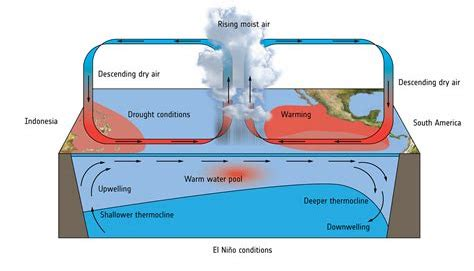
\includegraphics[width=.9\linewidth]{./images/el_nino_reduced.jpg}
\caption{Changes to tropical Pacific climate during El Niño. \url{https://www.esa.int/ESA\_Multimedia/Images/2018/08/El\_Nino}}
\end{figure}
\end{block}

\begin{block}{Long-Term vs Short-Term Chang}
\begin{itemize}
\item Long-term change: climate change/global warming
\begin{itemize}
\item Causes: greenhouse gasses, aerosols (smoke), land use, etc.
\end{itemize}
\item Short-term change: climate variability
\begin{itemize}
\item ENSO, seasons, AMO (Atlantic Multidecadal Oscillation), etc.
\end{itemize}
\end{itemize}

\begin{figure}[htbp]
\centering
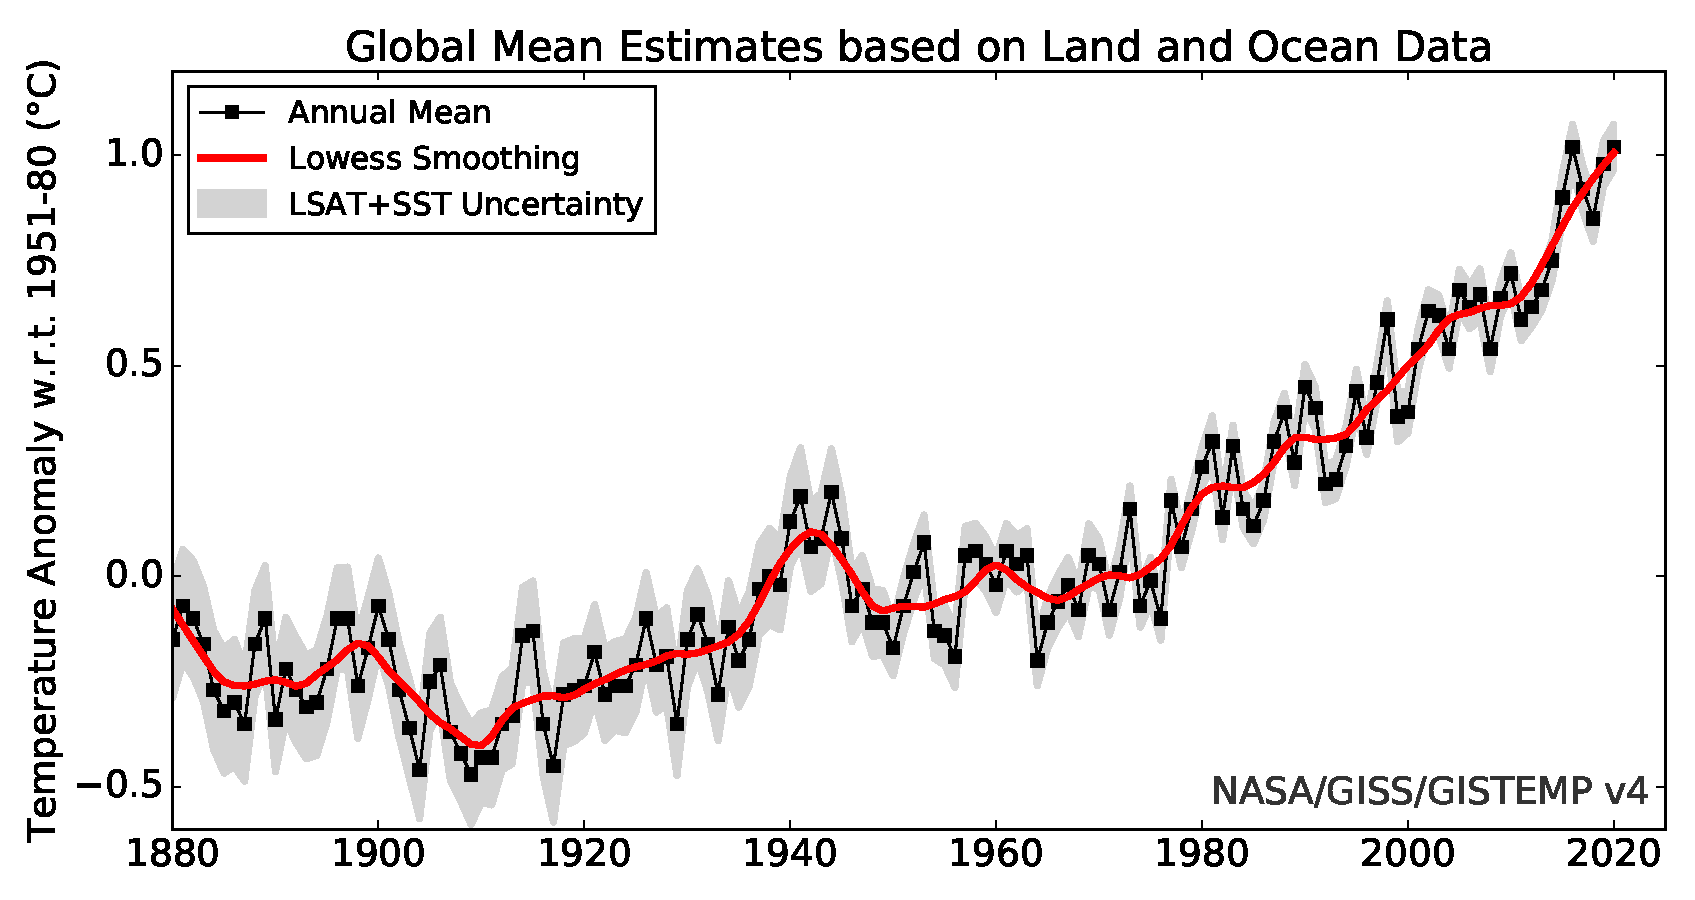
\includegraphics[width=.9\linewidth]{./images/climate_change.pdf}
\caption{Global average temperature changes since 1880. Red line: smoothed average, black line: unsmoothed average. \url{https://data.giss.nasa.gov/gistemp/graphs\_v4}}
\end{figure}
\end{block}

\begin{block}{Review of literature}
\begin{itemize}
\item \citet{chen2017possible}
\begin{itemize}
\item Past studies disagree about whether ENSO will strengthen or weaken.
\item Simulation discrepancy caused by modeling of ENSO mechanics.
\end{itemize}
\item \citet{maher2018enso}
\begin{itemize}
\item Used a large dataset of climate predictions.
\item ENSO may become stronger in the future.
\end{itemize}
\item \citet{cai2018increased}
\begin{itemize}
\item Found that models agree by using a more flexible way of defining ENSO events
\item ENSO is strengthening because global warming is leading to higher stratification.
\end{itemize}
\end{itemize}
\end{block}

\begin{block}{Research Goals}
\begin{itemize}
\item Overall changes to ENSO amplitude
\begin{itemize}
\item Estimate future changes to ENSO amplitude using the CESM1 dataset.
\end{itemize}
\item Role of individual factors
\begin{itemize}
\item Compare contributions of greenhouse gasses, aerosols, land use, biomass burning, and ozone to ENSO intensity.
\end{itemize}
\item Changes to ocean structure
\begin{itemize}
\item Examine changes to correlation coefficient between ENSO intensity and ocean temperature for each simulation.
\end{itemize}
\end{itemize}
\end{block}

\begin{block}{Data: the CESM1 Large Ensemble}
\begin{itemize}
\item Explore hypothetical scenarios with a computer model \citet{kay2015community}.
\item Estimation of how the earth's climate actually works.
\item Experimental group: Receives input of rising greenhouse gas and/or aerosol levels.
\item Control group: Emissions fixed at levels before industrial revolution.
\end{itemize}
\end{block}
\end{block}
\end{column}

\begin{column}{0.01\columnwidth}
\end{column}
\begin{column}{0.48\columnwidth}
\begin{block}{Methods}
\begin{columns}
\begin{column}{0.48\columnwidth}
\begin{block}{Niño 3.4 Variance}
\begin{itemize}
\item How to calculate ENSO intensity in the model output?
\item Step 1: Calculate sea temperature in Niño 3.4 region (5°N - 5°S, 120°-170°W) of tropical Pacific Ocean.
\item Step 2: Convert temperature dataset to dataset representing change in temperature variation over time.
\item Calculate variance around one point, move point forward slightly, repeat.
\end{itemize}
\end{block}

\begin{block}{Butterfly Effect: The Need for a Large Ensemble}
\begin{itemize}
\item Butterfly effect: Small differences in initial conditions can become big differences in end result \citep{lorenz1963deterministic}.
\item Each simulation by itself is inaccurate.
\item Repeat simulation with slightly different initial conditions.
\item Due to larger sample size, noise can be filtered out by calculating the mean.
\end{itemize}

\begin{figure}[htbp]
\centering
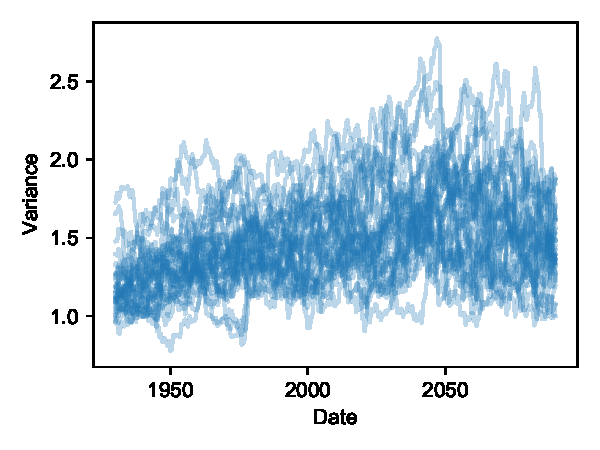
\includegraphics[width=.9\linewidth]{./images/variance_3.pdf}
\caption{Niño 3.4 20-year variance for individual members in full forcing ensemble.}
\end{figure}
\end{block}

\begin{block}{Model Predictions: ENSO in the Future}
\begin{itemize}
\item Calculate mean and standard error of ENSO intensity in ensemble and control.
\item ENSO is predicted to intensify in the 21st century!
\item Statistically significant: exceeds 2 standard errors.
\item Decreasing variance after 2060: still under investigation.
\end{itemize}

\begin{figure}[htbp]
\centering
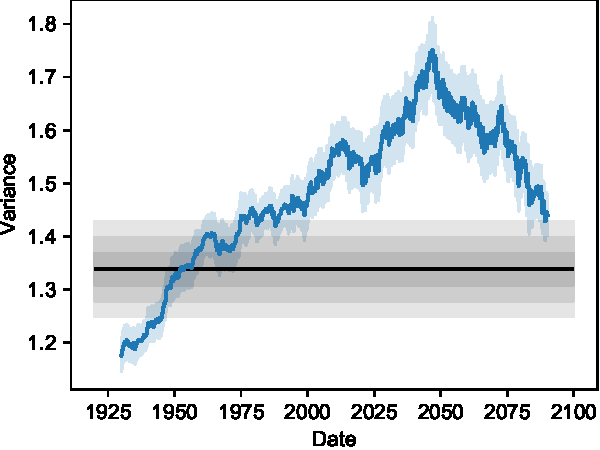
\includegraphics[width=.9\linewidth]{./images/variance_2.pdf}
\caption{20-year variance of Niño 3.4 index for fully-forced ensemble. Grey bar shows control mean and standard errors}
\end{figure}
\end{block}
\end{column}

\begin{column}{0.01\columnwidth}
\end{column}
\begin{column}{0.48\columnwidth}
\begin{block}{Analysis of Individual Factors}
\begin{itemize}
\item Why is ENSO predicted to intensify? What human impacts play the largest role?
\begin{itemize}
\item Factors include: Greenhouse gasses, aerosols, natural factors.
\end{itemize}
\item Separate out individual influences in model output.
\item Single forcing ensembles: forced by all factors except for 1.
\item Subtract “all-but-one” ensembles from original “full-forcing” ensemble.
\item Resulting data represents influence of only one factor.
\end{itemize}
\end{block}

\begin{block}{Role of Greenhouse and Aerosol Emissions}
\begin{itemize}
\item Greenhouse gasses and aerosols contribute to increase in variance.
\item Aerosols and greenhouse gasses have same sign: disagree with previous studies \citep{deser2020isolating}.
\item Greenhouse gasses and aerosols are both human-produced.
\end{itemize}

\begin{figure}[htbp]
\centering
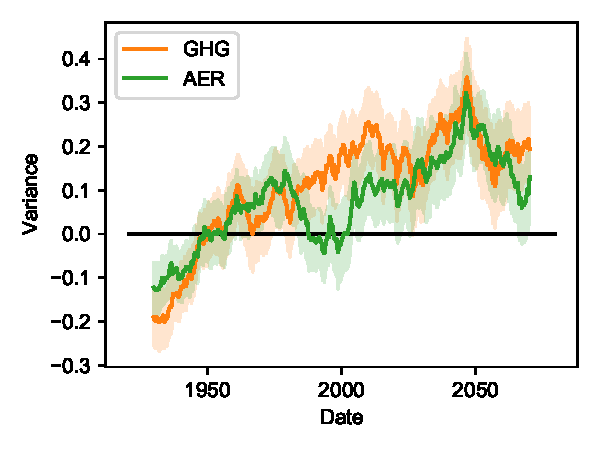
\includegraphics[width=.9\linewidth]{./images/bootstrap_2.pdf}
\caption{Influence of individual human factors. Yellow is greenhouse gasses, green is aerosols.}
\end{figure}
\end{block}

\begin{block}{Correlation With Changes in Ocean Temperature}
\begin{itemize}
\item Examine relationship between ocean temperature and ENSO intensity in each simulation.
\item Calculate correlation coefficient between ENSO intensity and ocean temperature.
\item Find correlation coefficient at each grid-point.
\end{itemize}
\end{block}

\begin{block}{Physical Mediator: Heating Difference}
\begin{itemize}
\item Strong negative correlation in fully forced ensemble below surface.
\item Positive correlation in greenhouse ensemble and weak/zero correlation in aerosols ensemble
\item Rising temperatures heat different layers of ocean at different rates, modifying heat transfer.
\end{itemize}

\begin{figure}[htbp]
\centering
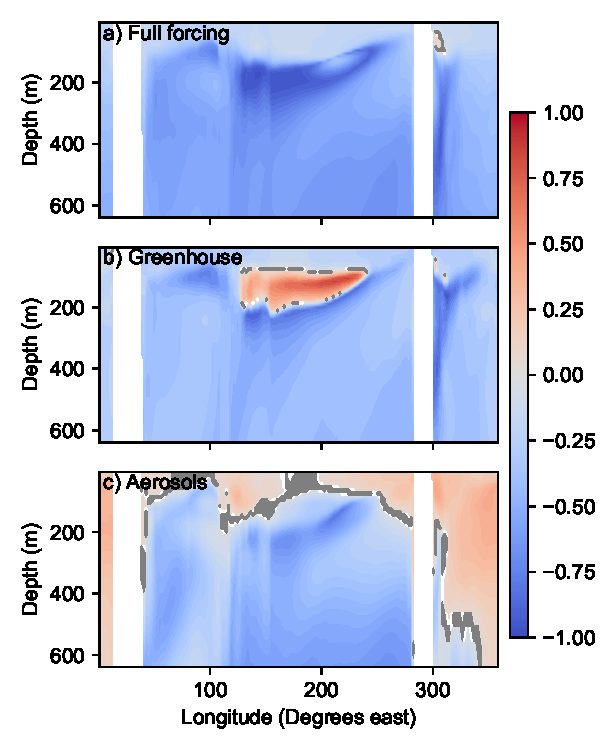
\includegraphics[width=.9\linewidth]{./images/diff_tempdt.pdf}
\caption{Correlation between ENSO intensity and ocean temperature in 3 major ensembles}
\end{figure}
\end{block}
\end{column}
\end{columns}
\end{block}
\end{column}

\begin{column}{0.01\columnwidth}
\end{column}
\begin{column}{0.24\columnwidth}
\begin{block}{Conclusion and Discussion}
\begin{itemize}
\item Predicted increase in variance
\begin{itemize}
\item There is likely to be an increase in ENSO strength over the next 100 years. Agrees with \citet{cai2018increased}.
\end{itemize}
\item Greenhouse gasses and aerosols
\begin{itemize}
\item Increase is likely caused by the combined influence of greenhouse gasses and aerosols.
\end{itemize}
\item Heat transfer
\begin{itemize}
\item Global warming increases ENSO intensity by warming upper layers of the Pacific faster than central layers.
\end{itemize}
\item Notable disagreement
\begin{itemize}
\item Greenhouse gasses and aerosols both increase ENSO amplitude, in contrast to \citet{deser2020isolating}
\end{itemize}
\end{itemize}
\end{block}

\begin{block}{Applications, Next Steps, Limitations}
\begin{itemize}
\item Improve prediction ability to help people prepare for increased likelihood of extreme weather.
\item Reduce danger by switching to renewable energy.
\item Limitations:
\begin{itemize}
\item Only used one climate model.
\item Niño 3.4 index may not be fully accurate for various models (Cai et. al. 2018).
\end{itemize}
\item Next steps:
\begin{itemize}
\item Work with other datasets, such as the new CESM2.
\item Examine other variables to further analyze mediator process.
\end{itemize}
\end{itemize}
\end{block}

\begin{block}{Acknowledgements}
\begin{itemize}
\item This material is based upon work supported by the National Center for Atmospheric Research, which is a major facility sponsored by the National Science Foundation under Cooperative Agreement No. 1852977.
\item Thank you to my teacher, my family, and my mentor!
\item Role of mentor:
\begin{itemize}
\item Provide raw data from his facility
\item Suggest methods and interpretations
\item Provide feedback on results
\item Make similar calculations to check student's results
\end{itemize}
\end{itemize}
\end{block}

\begin{block}{References}
\bibliographystyle{apa}
\fontsize{7pt}{7.2}\selectfont
\bibliography{references}
\end{block}
\end{column}

\begin{column}{0.01\columnwidth}
\end{column}
\end{columns}
\end{frame}
\end{document}
